\documentclass[]{standalone}

\usepackage{amsmath}
\usepackage{amsfonts}
\usepackage{amssymb}
\usepackage{graphicx}
\usepackage{tikz}
\usepackage{import}
\usepackage[subpreambles=true]{standalone}

\usepackage{tikz}
\usepackage{tikz-3dplot}
\usepackage{tikz_utils}

\usetikzlibrary{calc}
\usetikzlibrary{positioning}
\usetikzlibrary{patterns}
\usetikzlibrary{decorations,backgrounds}
\usetikzlibrary{angles,calc,positioning}
\usetikzlibrary{decorations.pathreplacing}
\usetikzlibrary{spy}

\begin{document}

\fontsize{8}{12}\selectfont

\begin{tikzpicture}[scale=1, anchor=mid]
    \coordinate (x) at (0,0,0);
    \coordinate (y) at (0.3,0,0);
    \coordinate (w) at (0.6,0,0);
    \coordinate (h) at (0.9,0,0);
    \coordinate (c) at (1.2,0,0);
    \coordinate (image) at (4.3,-2);

    % Coordinate system
    % \draw[red] (0,0,0) -- (1,0,0);
    % \draw[green] (0,0,0) -- (0,1,0);
    % \draw[blue] (0,0,0) -- (0,0,1);

    \begin{scope}[spy using outlines={circle, connect spies}]

        % Bounding Box Tensor
        \draw[thin, contour=0.48\pgflinewidth, fill=orange!30] (x) ++(0,1,1.33) -- ++(0,-2,0) -- node[below] {$\boldsymbol{x}\mathstrut$} ++(0.3,0,0) -- ++(0,2,0) -- cycle;
        \draw[thin, contour=0.48\pgflinewidth, fill=orange!30] (x) ++(0.3,1,1.33) -- ++(0,-2,0) -- ++(0,0,-2.66) -- ++(0,2,0) -- cycle;
        \draw[thin, contour=0.48\pgflinewidth, fill=orange!30] (x) ++(0,1,1.33) -- ++(0.3,0,0) -- ++(0,0,-2.66) -- ++(-0.3,0,0) -- cycle;

        \draw[thin, contour=0.48\pgflinewidth, fill=orange!30] (y) ++(0,1,1.33) -- ++(0,-2,0) -- node[below] {$\boldsymbol{y}\mathstrut$} ++(0.3,0,0) -- ++(0,2,0) -- cycle;
        \draw[thin, contour=0.48\pgflinewidth, fill=orange!30] (y) ++(0.3,1,1.33) -- ++(0,-2,0) -- ++(0,0,-2.66) -- ++(0,2,0) -- cycle;
        \draw[thin, contour=0.48\pgflinewidth, fill=orange!30] (y) ++(0,1,1.33) -- ++(0.3,0,0) -- ++(0,0,-2.66) -- ++(-0.3,0,0) -- cycle;

        \draw[thin, contour=0.48\pgflinewidth, fill=orange!30] (w) ++(0,1,1.33) -- ++(0,-2,0) -- node[below] {$\boldsymbol{w}\mathstrut$} ++(0.3,0,0) -- ++(0,2,0) -- cycle;
        \draw[thin, contour=0.48\pgflinewidth, fill=orange!30] (w) ++(0.3,1,1.33) -- ++(0,-2,0) -- ++(0,0,-2.66) -- ++(0,2,0) -- cycle;
        \draw[thin, contour=0.48\pgflinewidth, fill=orange!30] (w) ++(0,1,1.33) -- ++(0.3,0,0) -- ++(0,0,-2.66) -- ++(-0.3,0,0) -- cycle;

        \draw[thin, contour=0.48\pgflinewidth, fill=orange!30] (h) ++(0,1,1.33) -- ++(0,-2,0) -- node[below] {$\boldsymbol{h}\mathstrut$} ++(0.3,0,0) -- ++(0,2,0) -- cycle;
        \draw[thin, contour=0.48\pgflinewidth, fill=orange!30] (h) ++(0.3,1,1.33) -- ++(0,-2,0) -- ++(0,0,-2.66) -- ++(0,2,0) -- cycle;
        \draw[thin, contour=0.48\pgflinewidth, fill=orange!30] (h) ++(0,1,1.33) -- ++(0.3,0,0) -- ++(0,0,-2.66) -- ++(-0.3,0,0) -- cycle;

        \draw[thin, contour=0.48\pgflinewidth, fill=orange!30] (c) ++(0,1,1.33) -- ++(0,-2,0) -- node[below] {$\boldsymbol{c}\mathstrut$} ++(0.3,0,0) -- ++(0,2,0) -- cycle;
        \draw[thin, contour=0.48\pgflinewidth, fill=orange!30] (c) ++(0.3,1,1.33) -- ++(0,-2,0) -- node[below right] {$20$} ++(0,0,-2.66) -- node[right] {$15$} ++(0,2,0) -- cycle;
        \draw[thin, contour=0.48\pgflinewidth, fill=orange!30] (c) ++(0,1,1.33) -- ++(0.3,0,0) -- ++(0,0,-2.66) -- ++(-0.3,0,0) -- cycle;

        \path[fill=orange] ($(c) + (0.3,-1,1.33) + (0,0.8,-1.067)$) -- ++(0,0.133,0) -- ++(0,0,-0.133) -- ++(0,-0.133,0) -- cycle;

        \draw[thick, ->] ($(c) + (0.3, -1,1.33) + (0,0.866,-1.133)$) to node[below]{$c_{ij}>0.5$}++ (2.5,0);

        \node[inner sep=0pt, anchor=south west, draw opacity=0.5] at ($(image)$) {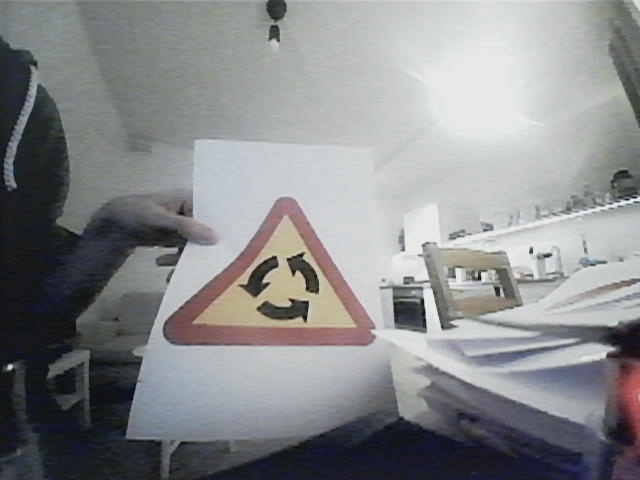
\includegraphics[width=6cm]{neural_network/image.jpg}};
        \foreach \i in {0,...,15}
        {
            \draw ($(image) + (0,0.3*\i)$) -- ++ (6,0);
        }
        \foreach \i in {0,...,20}
        {
            \draw ($(image) + (0.3*\i,0)$) -- ++ (0,4.5);
        }
        \draw[thick,orange] ($(image) + (2.4,1.8)$) --++ (0.3,0) -- ++ (0,0.3) -- ++(-0.3,0) -- cycle;

        \draw[red, thick] (image) ++ (1.53,1.26) rectangle ++ (1.98,1.41);
        \draw[red, |<->|] (image) ++ (1.53,1.26) ++ (0,-0.2) -- node[below]{$640 w_{ij}$}  ++ (1.98,0);
        \draw[red, |<->|] (image) ++ (1.53,1.26) ++ (-0.2,0) -- node[left]{$480 h_{ij}$} ++ (0,1.41);

        % \draw[red, <->] (image) ++ (1.53,1.26) ++ (0,0) -- node[below]{$640/20 x_{ij}$}  ++ (1.98,0);
        % \draw[red, <->] (image) ++ (1.53,1.26) ++ (2,0) -- node[left]{$480/15 y_{ij}$} ++ (0,1.41);

        \path[orange, fill] (image) ++ (1.53,1.26) ++ (0.99, 0.705) coordinate (center) circle (0.02);
        
        \spy[size=2.5cm, thick,magnification=4] on (center) in node (s) at (8.5,1.5);

    \end{scope}

    \draw[red, <->] (s.center) -- node[below]{$\frac{640}{20}x_{ij}$} ++ (-0.48,0);
    \draw[red, <->] (s.center) -- node[right]{$\frac{480}{15}y_{ij}$} ++ (0,0.54);

%     \draw[thick] ($(image_b) + (0.3,0,0)$) -- (mobilenet);


%     % MobileNetV2
%     \draw[thin, contour=0.48\pgflinewidth, fill=white] (mobilenet) ++(0,0.6,0.6) -- ++(0,-1.2,0) -- ++(3,0,0) -- ++(0,1.2,0) -- cycle;
%     \draw[thin, contour=0.48\pgflinewidth, fill=white] (mobilenet) ++(3,0.6,0.6) -- ++(0,-1.2,0) -- ++(0,0,-1.2) -- ++(0,1.2,0) -- cycle;
%     \draw[thin, contour=0.48\pgflinewidth, fill=white] (mobilenet) ++(0,0.6,0.6) -- ++(3,0,0) -- ++(0,0,-1.2) -- ++(-3,0,0) -- cycle;
%     \node at ($(mobilenet) + (1.5, 0 ,0.6)$) {MobileNetV2};

%     \draw[thick] ($(mobilenet) + (3,0,0)$) -- (feature);

%     \draw[thin, contour=0.48\pgflinewidth, fill=orange!30] (feature) ++(0,0.6,0.8) -- ++(0,-1.2,0) -- node[below] {$1280$} ++(3,0,0) -- ++(0,1.2,0) -- cycle;
%     \draw[thin, contour=0.48\pgflinewidth, fill=orange!30] (feature) ++(3,0.6,0.8) -- ++(0,-1.2,0) -- node[below right] {$20$} ++(0,0,-1.6) -- node[right] {$7$} ++(0,1.2,0) -- cycle;
%     \draw[thin, contour=0.48\pgflinewidth, fill=orange!30] (feature) ++(0,0.6,0.8) -- ++(3,0,0) -- ++(0,0,-1.6) -- ++(-3,0,0) -- cycle;

%     \node at ($(feature) + (1.5, -0.6, 0.8) + (0, -0.7, 0)$) {Feature Tensor};

%     \draw[thick] ($(feature) + (3,0,0)$) -- (conv);

%     \draw[thin, contour=0.48\pgflinewidth, fill=white] (conv) ++(0,0.2,0.2) -- ++(0,-0.4,0) -- ++(3,0,0) -- ++(0,0.4,0) -- cycle;
%     \draw[thin, contour=0.48\pgflinewidth, fill=white] (conv) ++(3,0.2,0.2) -- ++(0,-0.4,0) -- ++(0,0,-0.4) -- ++(0,0.4,0) -- cycle;
%     \draw[thin, contour=0.48\pgflinewidth, fill=white] (conv) ++(0,0.2,0.2) -- ++(3,0,0) -- ++(0,0,-0.4) -- ++(-3,0,0) -- cycle;
%     \node at ($(conv) + (1.5, 0 ,0.2)$) {$1\times 1$ Conv};

%     \draw[thick, decorate,decoration={brace,amplitude=3pt}] ($(conv) + (-0.1, 0.4, 0)$) -- node[above=0.1] {Head} ++ (3.3,0,0); 

%     \draw[thick] ($(conv) + (3,0,0)$) -- (bbs);

%     \draw[thin, contour=0.48\pgflinewidth, fill=orange!30] (bbs) ++(0,0.6,0.8) -- ++(0,-1.2,0) -- node[below] {$5$} ++(0.5,0,0) -- ++(0,1.2,0) -- cycle;
%     \draw[thin, contour=0.48\pgflinewidth, fill=orange!30] (bbs) ++(0.5,0.6,0.8) -- ++(0,-1.2,0) -- node[below right] {$15$} ++(0,0,-1.6) -- node[right] {$7$} ++(0,1.2,0) -- cycle;
%     \draw[thin, contour=0.48\pgflinewidth, fill=orange!30] (bbs) ++(0,0.6,0.8) -- ++(0.5,0,0) -- ++(0,0,-1.6) -- ++(-0.5,0,0) -- cycle;

%     \node[align=center] at ($(bbs) + (0.25, -0.6, 0.8) + (0, -0.7, 0)$) {Bounding Box Tensor};

%     \draw[thick, decorate,decoration={brace,amplitude=3pt}] ($(mobilenet) + (-0.2, 1, 0)$) -- node[above=0.1] {Backbone} ++ (3.6,0,0); 

    % \draw[thin, contour=0.48\pgflinewidth, fill=green!30] (image_g) ++(0,0.6,0.9) -- ++(0,-1.2,0) -- ++(0.2,0,0) -- ++(0,1.2,0) -- cycle;
    % \draw[thin, contour=0.48\pgflinewidth, fill=green!30] (image_g) ++(0.2,0.6,0.9) -- ++(0,-1.2,0) -- ++(0,0,-1.8) -- ++(0,1.2,0) -- cycle;
    % \draw[thin, contour=0.48\pgflinewidth, fill=green!30] (image_g) ++(0,0.6,0.9) -- ++(0.2,0,0) -- ++(0,0,-1.8) -- ++(-0.2,0,0) -- cycle;

    % \draw[thin, contour=0.48\pgflinewidth, fill=blue!30] (image_b) ++(0,0.6,0.9) -- ++(0,-1.2,0) -- ++(0.2,0,0) -- ++(0,1.2,0) -- cycle;
    % \draw[thin, contour=0.48\pgflinewidth, fill=blue!30] (image_b) ++(0.2,0.6,0.9) -- ++(0,-1.2,0) -- ++(0,0,-1.8) -- ++(0,1.2,0) -- cycle;
    % \draw[thin, contour=0.48\pgflinewidth, fill=blue!30] (image_b) ++(0,0.6,0.9) -- ++(0.2,0,0) -- ++(0,0,-1.8) -- ++(-0.2,0,0) -- cycle;
    
\end{tikzpicture}

\end{document}
